\documentclass[12pt]{article}
\usepackage[brazil]{babel}
\usepackage{graphicx}
\usepackage{mathtools}
\usepackage{float} 
\usepackage{xcolor}


\usepackage{array}
\usepackage{booktabs}



% margenes
\usepackage[a4paper,left=2cm,right=2cm,top=1cm]{geometry}

%opening
\title{\textbf{Modelagem de Escoamentos Turbulentos. \\Lista de Exercícios No. 2}}

\author{Cristian Herledy López Lara}
\date{Junho 2025}

\begin{document}
	
\maketitle


\section*{Questão 1}

A partir do conjunto de dados fornecido no arquivo Re125.txt para a velocidade instantânea
medida em um ponto de um jato (coluna 1: tempo em segundos; coluna 2: velocidade em
m/s), e considerando amostras para intervalos de tempo T = 0,005; 0,05; 0,5 e 5s:\\
i. Obtenha a velocidade média e desvio padrão;\\
ii. Explique eventuais diferenças entre os resultados para os três períodos T supracitados.\\


\textbf{\underline{Desenvolvimento}}

A velocidade média e o desvio padrão são calculados para cada intervalo mostrando os seguintes valores:

\begin{table}[h]
	\centering
	\begin{tabular}{|c|c|c|}
		\hline
		Periodo T [s] & U media [m/s] & Desvio padrão [m/s]; \\ \hline
		0 - 0,005   & 8,8854    & 1,0636    \\ \hline
		0 - 0,05   & 8,5692   & 1,1724  \\ \hline
		0 - 0,5    & 8,5342    & 1,2415    \\ \hline
		0 - 5    & 8,5417    & 1,2330   \\ \hline
	\end{tabular}
	\caption{Valores de velocidade media e desvio padrão para diferentes intervalos}
\end{table} 

\begin{figure}[H]
	\centering
	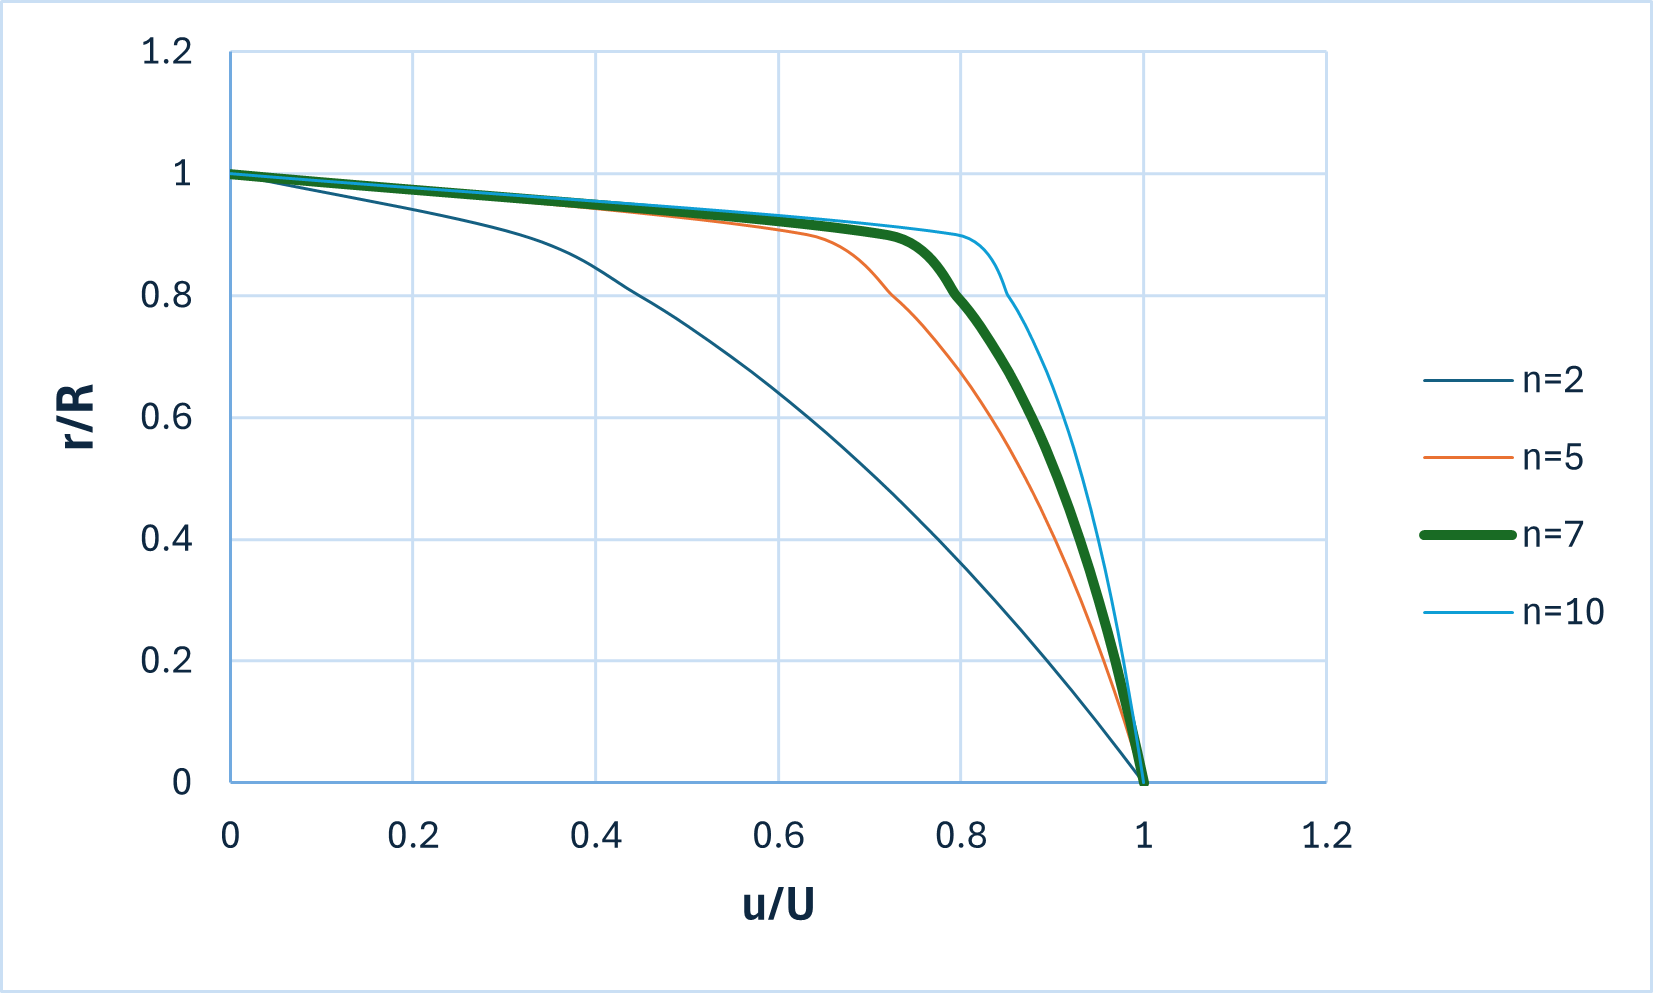
\includegraphics[width=.65\textwidth]{figures/1}
	\caption{Velocidade instantanea e velocidade media ate $t=0,05s$}
\end{figure}

O gráfico a seguir mostra a evolução da velocidade média e do desvio padrão. Ambas as grandezas convergem para um valor à medida que o tempo avança. Isso ocorre porque há mais dados para calcular a média da amostra em $t=5s$. As grandes e pequenas escalas terão passado pelo dispositivo de medição um número maior de vezes, o que permite estatísticas turbulentas mais homogêneas e, portanto, a medição do escoamento em regime permanente.

\begin{figure}[H]
	\centering
	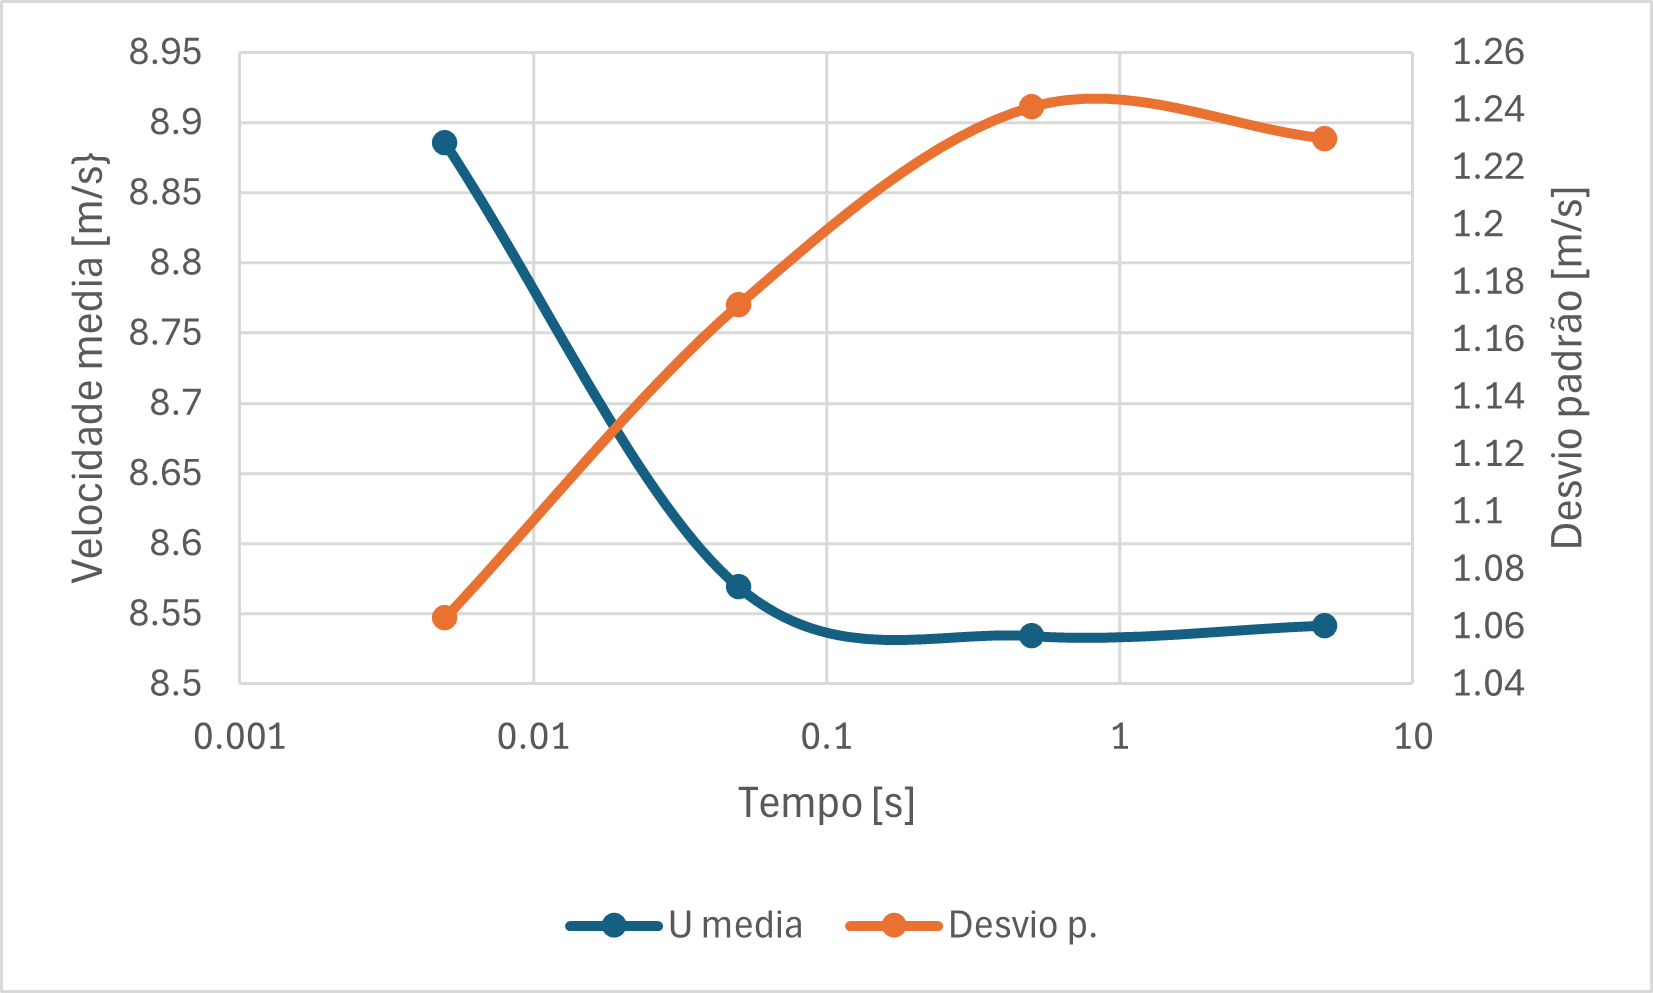
\includegraphics[width=.65\textwidth]{figures/2}
	\caption{Velocidade media e desvio padrao nos intervalos de tempo analisados}
\end{figure}


\section*{Questão 2}

A partir dos dados do arquivo Re125.txt:\\
\textbf{i. Determine a energia cinética turbulenta, k, assumindo a condição de isotropia;}\\

A energia cinética turbulenta é calculada com a expressão


\begin{equation}
	k = {\overline{u_i u_i}}/2
\end{equation}
Que para un escoamento isotrópico pode ser escrito como 

\begin{equation}
	k = {\overline{u1u1 + u1u1 + u1u1}}/2 \ = \ \frac{3}{2}\overline{u_1 u_1}^2 \ = \ 2,26 \ \frac{m^2}{s^2}
\end{equation}

\textbf{ii. Faça um gráfico para o coeficiente de correlação temporal e avalie a escala de
comprimento L das grandes escalas;}\\

Para o cálculo de correlação temporal , primeiro é necesario encomtrar o valor da correlação de velocidade no ponto $(r=0)$ dado pela expressão


\begin{equation*}
	\mathbf{R}_{ij}^{(t)}(\mathbf{x}, \boldsymbol{\tau}) = \overline{u_i(\mathbf{x}, t) \, u_j(\mathbf{x}, t')}
\end{equation*}


Sendo $\tau = t - t'$. Logo, a correlação de velocidades é calculada como 

\begin{equation}
	\rho_{ij}^{(t)}(\mathbf{x}, \boldsymbol{\tau}) = 
	\frac{\mathbf{R}_{ij}^{(t)}(\mathbf{x}, \boldsymbol{\tau})}
	{u_i' u_j'}
\end{equation}

Para finalmente determinar a correpondente correlação temporal

\begin{equation}
	\Theta_{ij} = \int_{-\infty}^{+\infty} \rho_{ij}^{(t)}(\mathbf{x}, \boldsymbol{\tau}) \, \mathrm{d} \boldsymbol{\tau}
\end{equation}

O gráfico a seguir mostra como se comporta a correlação temporal em uma parcela da amostra de dados selecionada até $\tau = 0,02$, já que com todos os dados não é fácil visualizar a tendência da curva.

\begin{figure}[H]
	\centering
	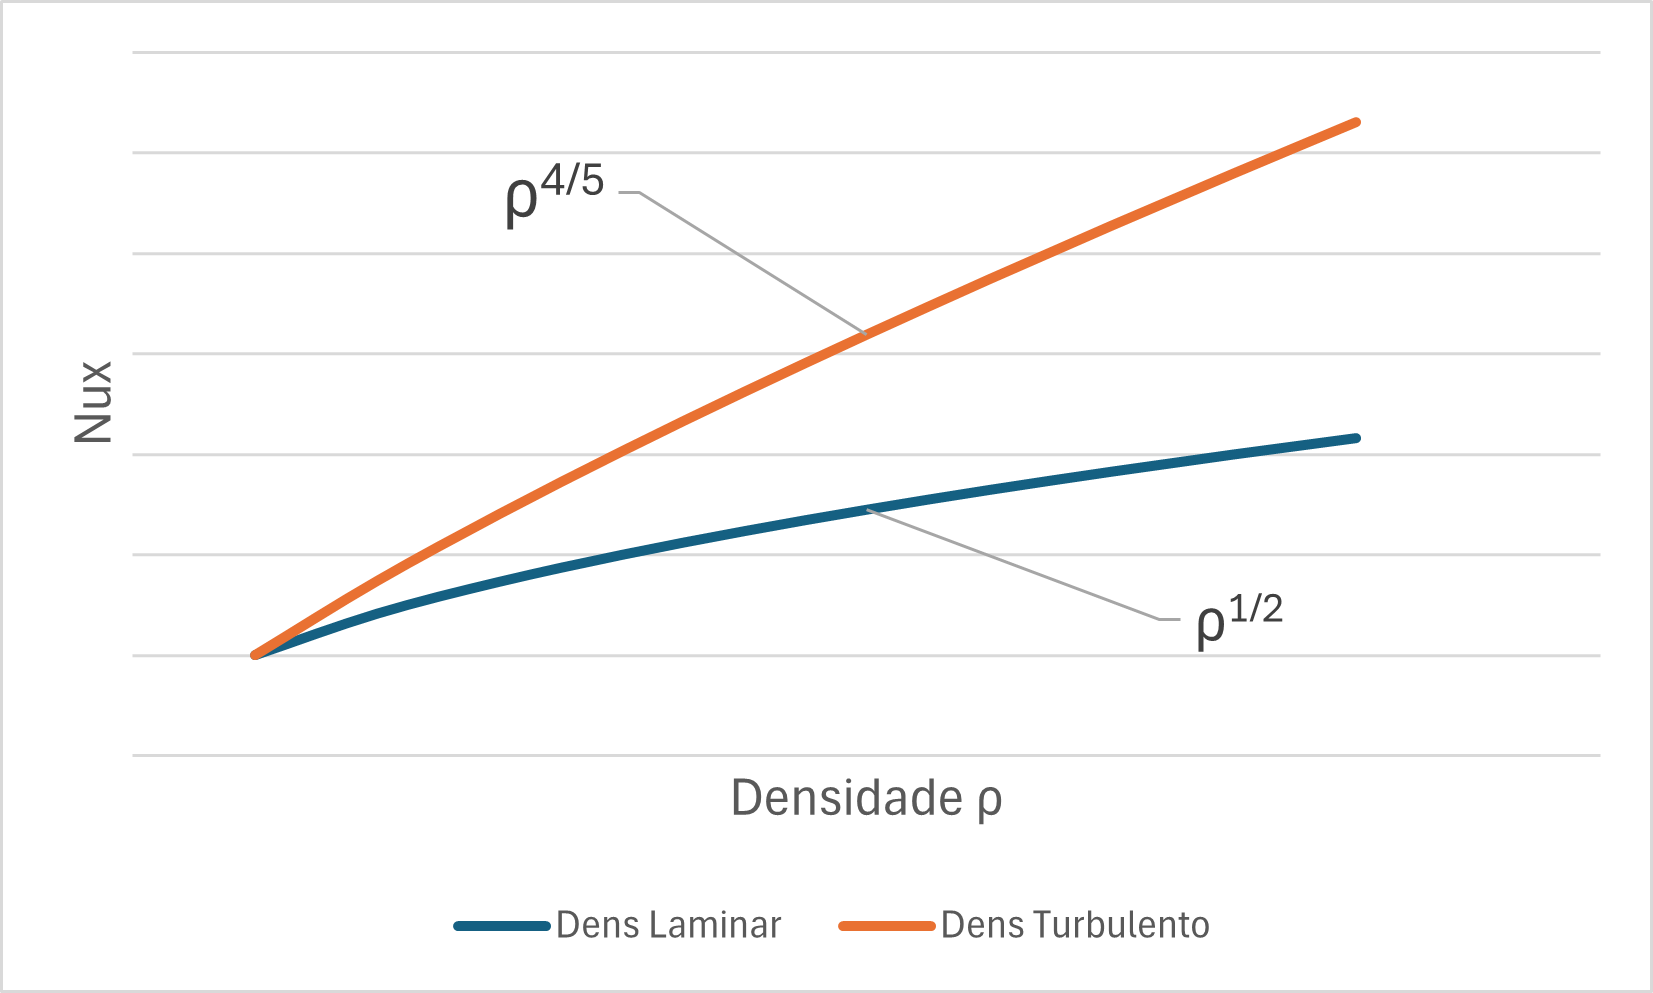
\includegraphics[width=.65\textwidth]{figures/3}
	\caption{Evolução da correlação temporal em função de $\tau$}
\end{figure}

Para determinar o valor da escala de comprimento para grandes escalas $L$, são tomados valores positivos da expressão (4) levando a sua forma integral ao calculo pelas somas em serie; uma vez que esses valores positivos correspondem à correlação direta das flutuações com o atraso. Este valor representa o tempo médio de passagem das estruturas turbulentas pelo dispositivo de medição. \\

Segregando o primeiro intervalo de valores positivos $ \Theta_1 $ no intervalo da figura 3, obtém-se a curva

\begin{figure}[H]
	\centering
	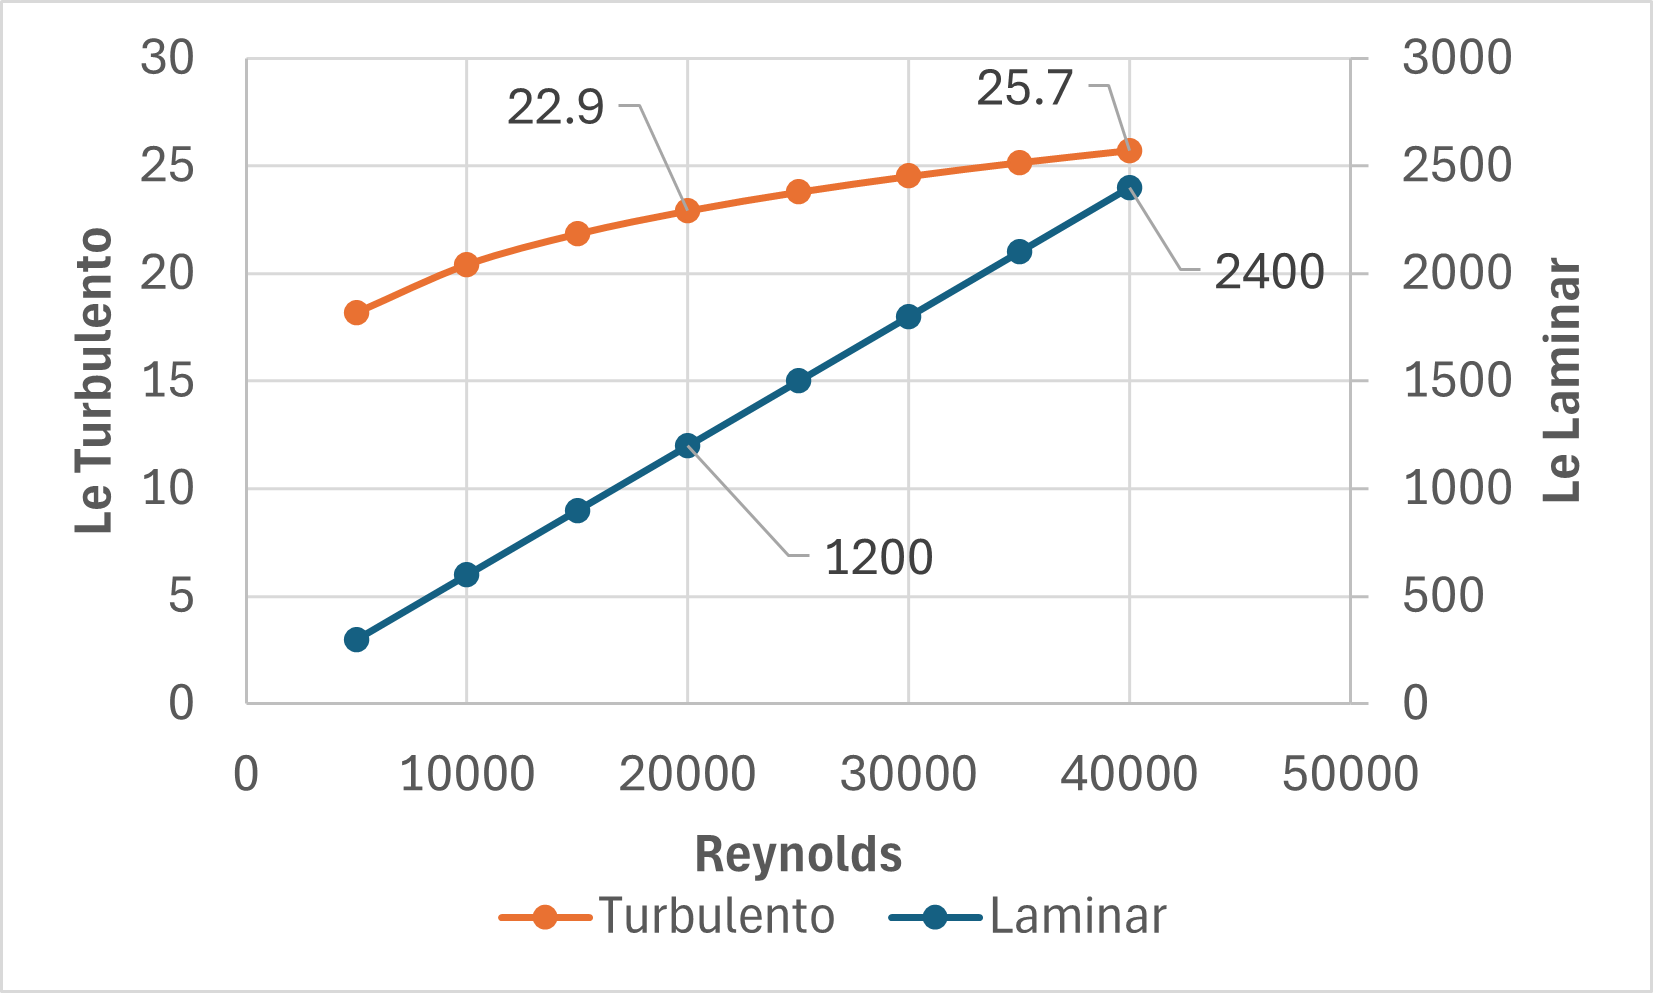
\includegraphics[width=.65\textwidth]{figures/4}
	\caption{Evolução da correlação temporal ate $\Theta_1 = 0$}
\end{figure}

Agora, da seguinte expressão, L pode ser calculada

\begin{equation}
	\Theta = \frac{L}{U} \ \rightarrow \ L = 0,003059 \ m
\end{equation}

\textbf{iii. Avalie o número de Reynolds das grandes escalas, ReL, a partir das medições}\\

O número de Reynolds é avaliado, tomando o valor da viscosidade do ar @ $298,15 K$

\begin{equation}
	Re_L = \frac{u' \cdot L}{\nu} = \frac{1,2330 m/s \cdot 0,0030m}{1,5e^{-5} m^2/s } \ = \ 251,5
\end{equation}

\textbf{iv. Obtenha estimativas paras as escalas de Kolmogorov (comprimento, tempo e
velocidade)\\
v. Avalie a dissipação turbulenta}\\

Para avaliar as escalas de Kolmogorov e a dissipação turbulenta as seguintes considerações serão feitas para usar a nomenclatura das equações da aula
\begin{itemize}
	\item $\ell_0 = L$
	\item $u_0 = u'$
	\item $\tau_0 = \ell_0 / u_0$
\end{itemize}


\begin{equation}
	\varepsilon \equiv \frac{(u_0)^3}{\ell_0} \ \equiv \frac{(1,2330 m/s)^3}{0,0030m} \ \equiv \ 625 m^2/s^3
\end{equation}

\begin{equation}
	\frac{\eta}{\ell_0} \sim Re_L^{-3/4} \ \rightarrow \ \eta  \sim Re_L^{-3/4} \cdot \ell_0 \ \rightarrow \ 251,5^{-3/4} \cdot 0,0030m \sim 4,84 x 10^-5 m 
\end{equation}

\begin{equation}
	\frac{u_\eta}{u_0} = Re_L^{-1/4} \rightarrow u_\eta= Re_L^{-1/4} \cdot u_0 \rightarrow 251,5^{-1/4} \cdot 1,2330 m/s = 0,3096 m/s
\end{equation}

\begin{equation}
	\frac{\tau_\eta}{\tau_0} = Re_L^{-1/2} \rightarrow \tau_\eta = Re_L^{-1/2} \cdot \tau_0 \rightarrow 251,5^{-1/2} \cdot 0,0024 s = 1,51x10^{-4} s
\end{equation}

Em resumo das escalas de Kolmogorov obtem-se que:
\begin{itemize}
	\item $\varepsilon \equiv 625 m^2/s^3 $
	\item $\eta = 4,84 x 10^-5 m$
	\item $u_\eta = 0,3096 m/s$
	\item $\tau_\eta = 1,51x10^{-4} s$
\end{itemize}

Os resultados obtidos refletem o regime turbulento de grandes escalas, onde $Re>1$ mostra que grandes estruturas contêm uma grande parcela da energia inercial.\\
A dissipação turbulenta mostra a taxa de transferência de energia para as escalas viscosas.

O valor de $\ell_0$ é consistente com a escala de comprimento que divide a faixa inercial da faixa dissipativa $\ell_{DI} = 60 \eta \rightarrow 0,0030 m \approx 60\cdot  4,84 x 10^-5 m  $. Este valor é necessário para definir a escala para a segunda hipótese de similaridade.

A velocidade $u_\eta$ e muito menor que as velocidades media e de fluctuação. Isso da uma ideia sobre como escalas grandes e pequenas se desacoplaram.

O tempo característico das pequenas estruturas $\tau_\eta$ é significativamente menor que o tempo integral $\tau_0$, mostrando que a dissipação ocorre rapidamente. \\
\textbf{vi. Determine a transformada de Fourier para energia cinética instantânea da turbulência e
forneça uma interpretação do resultado, identificando as faixas de energia, inercial e de
dissipação das escalas turbulentas.}

\begin{figure}[H]
	\centering
	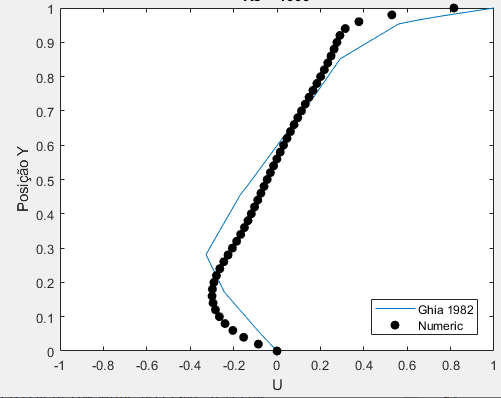
\includegraphics[width=.65\textwidth]{figures/6}
	\caption{Transformada de Fourier para energia cinética instantânea da turbulência}
\end{figure}

As divisões das diferentes regiões podem ser vistas no anterior grafico.
A transição da faixa de energia (onde a maior parte da energia turbulenta está contida) concorda com a relação ao intervalo $\ell_0/6 < \ell < 6\ell_0$, começando em torno de 1200 Hz. Nessa faixa, ocorre a produção de energia turbulenta que será trasnferida as pequenas escalas passando pela faixa inercial.

En tanto, a região de dissipação cobre $\approx 60\%$ do espectro, sendo esta a faixa onde ocorre a dissipação de energia das pequenas escalas ao escoamento. Para os dados analisados, o limite para esta região é da ordem de $10^2$ Hz, o que coincide com a expressão dada para $\ell_{DI}$.

A região inercial (em amarelo) é o intervalo de frequências onde ocorre a transferência de energia sem dissipação, da escala $L$ até escalas menores. Nesta faixa, o espectro tende a seguir a lei de Kolmogorov $\approx f^{-5/3}$:


\begin{thebibliography}{999}
	
	
	\bibitem{Deschamps}
	Cesar Deschamps,
	Escalas da turbulencia Cap 2.
	UFSC Florianopolis, SC,
	Notas de aula,
	2025.
		
	
\end{thebibliography}


\end{document}





